%\documentclass{iesbs}
\documentclass{amsart}
\usepackage{latexsym}
\usepackage{lscape}
\usepackage{graphics}
\usepackage{alltt}
\setcounter{secnumdepth}{3}
\setcounter{tocdepth}{3}
\setlength{\textwidth}{135mm}
\setlength{\textheight}{200mm}
\setlength{\oddsidemargin}{10mm}
\setlength{\evensidemargin}{10mm}
\setlength{\topmargin}{0mm}
\setlength{\textwidth}{6in}
\renewcommand{\abstractname}{Abstract}
\newtheorem{assumption}{Assumption}
\newtheorem{lemma}{Lemma}[section]
\newtheorem{theorem}{Theorem}[section]
\def\sT{\scriptscriptstyle T}
\def\RR{\hbox{\raise.4ex\hbox{$\scriptstyle{|}$}\hskip-1.85pt R}}
\def\OO{\mathcal O}
\def\SS{\mathcal S}
\def\argmin{\mathrm{argmin}}
\newcommand{\Jureckova}{Jure\v{c}kov\'{a} }
\newcommand{\Hajek}{H\'{a}jek }
\newcommand{\Hardle}{H\"{a}rdle }
\newcommand{\Sidak}{\v{S}id\'{a}k }

\newcommand{\C}{\mathbb C}
\newcommand{\R}{\mathbb R}
\newcommand{\N}{\mathbb N}
\newcommand{\Z}{\mathbb{Z}}

\newenvironment{apabib}{
  \noindent
\begin{center}
{\bf{ R}EFERENCES}
\end{center}
\vspace{-3mm}
\begin{list}{}{
  \topsep          0mm
  \leftmargin     10mm
  \parsep          0mm
  \listparindent -10mm}
  \item[]\strut\par}{
\end{list}}
 

\begin{document}
\title{\sc  Regression Quantiles }
%\thanks{
%Version: {\today}.
%This article has been prepared for the statistics section of the
%{\it International Encyclopedia of the Social Sciences}
%edited by Stephen Fienberg and Jay Kadane.
%The research was partially supported by NSF grant SBR-9617206.
%}



\author{\sc Roger Koenker*}
\thanks{*McKinley Professor of Economics and Statistics at the
University of Illinois at Urbana-Champaign}

\begin{abstract}
Classical least squares regression may be viewed as a
natural way of extending the idea of estimating an unconditional
mean parameter to the problem of estimating conditional mean {\it functions};
the crucial link is the formulation of an optimization problem
that encompasses both problems.  Likewise, quantile regression
offers an extension of univariate quantile estimation to estimation
of conditional quantile functions via an optimization of
a piecewise linear objective function in the residuals.  Median
regression minimizes the sum of absolute residuals, an idea introduced
by Boscovich in the 18th century. The asymptotic theory of quantile regression closely parallels the
theory of the univariate sample quantiles. Computation
of quantile regression estimators may be formulated as a linear
programming problem and efficiently solved by simplex or
barrier methods.  A close link to rank based inference has been
forged from the theory of the dual regression quantile process,
or regression rankscore process.
\end{abstract}

\maketitle

Quantile regression is a statistical technique intended to estimate,
and conduct inference about, conditional quantile functions. 
Just as classical linear regression methods based on
minimizing sums of squared residuals enable one to estimate models for
conditional mean functions, quantile regression methods offer a mechanism
for estimating models for the conditional median function, {\it and the full
range of other conditional quantile functions}.
By supplementing the estimation of conditional mean functions with
techniques for estimating an entire family of conditional quantile
functions, quantile regression is capable of providing a more
complete statistical analysis of the stochastic relationships among
random variables.

Quantile regression has been used in a broad range of application settings.
Reference growth curves for childrens' height and weight have a long history
in pediatric medicine; quantile regression methods may be used to estimate
upper and lower quantile reference curves as a function of age, sex, and
other covariates without imposing stringent parametric assumptions on the
relationships among these curves.  Quantile regression methods have been
widely used in economics to study determinents of wages, discrimination
effects, and trends in income inequality.  
Several recent studies have modeled the performance of public school
students on standardized exams as a function of socio-economic characteristics
like their parents' income and educational attainment, and policy variables 
like class size, school expenditures, and teacher qualifications.  It seems
rather implausible that such covariate effects should all act so as to
shift the entire distribution of test results by a fixed amount.
It is of obvious interest to know whether policy interventions alter
performance of the strongest students in the same way that weaker students
are affected.  Such questions are naturally investigated within the quantile
regression framework.  

 
\section{Quantiles, Ranks and Optimization}

We say that a student scores at the $\tau$th quantile
of a standardized exam if he performs {\it better} than the proportion $\tau$, 
and {\it worse} than the proportion $(1-\tau)$, 
of the reference group of students.
Thus, half of the students perform better than the median student, and half
perform worse.  Similarly, the quartiles divide the population into four 
segments with equal proportions of the population in each segment.  
The quintiles divide the population into 5 equal segments; the deciles
into 10 equal parts.  The quantile, or percentile, refers to the general case.

More formally, any real valued random variable, $Y$, 
may be characterized by its distribution function,
 $
F(y) = \mathrm{Prob}(Y  \leq  y)
$ 
while for any $0 < \tau < 1$, 
 $
Q ( \tau )  = \inf \{ y : F(y) \geq \tau \}
$ 
is called the $\tau$th quantile of $X$.
The median, $Q( 1/2 )$,  plays the central role.
Like the distribution function, the quantile function provides a
complete characterization of the random variable, Y.

The quantiles may be characterized as the solution to a  simple optimization 
problem.  For any $0 < \tau < 1$,  define the piecewise linear
``check function'', $\rho_\tau (u) = u ( \tau - I(u < 0 )) = \tau u^+ + (1-\tau )u^-$, where $u^+=u I[u>0]$ and  $u^-= -uI[u<0]$ denote the positive and negative parts, respectively,  of  $u\in\R$.  Minimizing the expectation of $\rho_\tau(Y-\xi)$ with respect to $\xi$
yields solutions, $\hat \xi (\tau)$, the smallest of which is $Q(\tau)$ defined
above.  

The sample analogue of $Q(\tau)$,
based on a random sample, $\{ y_1 , ... , y_n \}$, of $Y$'s, 
is called the $\tau$th {\it sample} quantile, and may be found by solving,
 $
\min_{\xi \in {\bf R}}  \sum_{i=1}^n \rho_{\tau} ( y_i - \xi ). 
$ 
While it is more common to define the sample quantiles in terms of 
the order statistics  $ y_{(1)} \leq y_{(2)} \leq ... \leq y_{(n)}$,
constituting a sorted rearrangement of the original sample, their
formulation as a minimization problem has the advantage that it
yields a natural generalization of the quantiles to the regression context.  

Just as the idea of estimating the unconditional mean, 
viewed as the minimizer,
\[
\hat \mu = \mathrm{argmin}_{\mu \in \RR} \sum (y_i - \mu)^2
\]
can be extended
to estimation of the linear conditional mean function $E(Y|X=x)=x' \beta$
by solving,
\[
\hat \beta = \mathrm{argmin}_{\beta \in \RR^p} \sum (y_i - x_i' \beta)^2 ,
\]
the linear conditional quantile function, $Q_Y(\tau | X=x) = x_i' \beta (\tau)$,
can be estimated by solving
\[
\hat \beta (\tau) = 
\mathrm{argmin}_{\beta \in \RR^p} \sum \rho_\tau (y_i - x' \beta).
\]
 
 The median case, $\tau = 1/2$, which is equivalent to minimizing the
sum of {\it absolute} values of the residuals 
has a long history, which goes back to  Boscovich  and  Laplace.  
The extension to quantiles other than the median was introduced in
Koenker and Bassett (1978), who also showed that $\hat \beta (\tau)$ can be obtained by  standard linear programming techniques. 


Robustness to distributional assumptions is another  important feature of regression quantile techniques. Quantile regression indeed  inherits certain robustness properties  of the ordinary 
sample quantiles.  The estimates and the associated inference apparatus have
an inherent distribution-free character since quantile estimation is
influenced only by the local behavior of the conditional distribution
of the response near the specified quantile.  
Given a solution $\hat \beta (\tau)$, based on observations, $\{y,X\}$,
as long as one doesn't alter the sign of the residuals, {\em any} of the $y$
observations may be arbitrary altered without altering the initial solution.  
Only the signs of the residuals matter in determining the quantile regression
estimates, and thus outlying responses influence the fit in so far as
they are either above or below the fitted hyperplane, but how far above or
below is irrelevant.
 
\section{An Example}

To illustrate the approach we may consider an analysis of a simple first order
autoregressive  model for maximum daily temperature in Melbourne, Australia.
The data are taken from Hyndman, Bashtannyk, and Grunwald (1996). 
In Figure 2 we provide a scatter plot of 10 years
of daily temperature data:  today's maximum daily temperature is plotted
against yesterday's maximum.  Our first observation from the plot is that there 
is a strong tendency for data to cluster along the (dashed) 45 degree line 
implying that with high probability today's 
maximum is near yesterday's maximum.  But closer examination of the
plot reveals that this impression is based primarily on the left side of the
plot where the central tendency of the scatter follows the 45 degree line
very closely.  On the right side, however, corresponding to summer conditions,
the pattern is more complicated.  There, it appears that {\it either}
there is another hot day, falling again along the 45 degree line, {\it or}
there is a dramatic cooling off.  But a mild cooling off appears to be more
rare.  In the language of conditional densities, if today is hot, tomorrow's
temperature appears to be bimodal with one mode roughly centered at today's
maximum, and the other mode centered at about $20^\circ$.
 
 
\begin{figure}
\begin{center}
\resizebox{\textwidth}{!}
{\includegraphics{fig.temp.3a.ps}}
\begin{caption}{Melbourne Maximum Daily Temperature:  The plot
illustrates 10 years of daily maximum  temperature data (in degrees centigrade)
for Melbourne, Australia as an AR(1) scatterplot.  
The data is scattered around the (dashed) 45 degree line suggesting
that today  is roughly similar to yesterday.  
Superimposed on the scatterplot 
are estimated conditional quantile functions for  the quantiles
$\tau \in \{ .05, .10, ... , .95 \}$.
Note that when yesterday's temperature is high the spacing between
adjacent quantile curves is narrower around the 45 degree line and
at about 20 degrees Centigrade than it is in the intermediate region.
This suggests bimodality of the conditional density in the summer.
}
\end{caption}
\label{temp2}
\end{center}
\end{figure}
 
  
Several estimated quantile regression curves have been superimposed
on the scatterplot.  Each curve is specified as a linear B-spline. 
Under winter conditions these curves are bunched around the 45 degree
line, however in the summer it appears that the upper quantile curves
are bunched around the 45 degree line and around $20^\circ$.  In the
intermediate temperatures the spacing of the quantile curves is somewhat
greater indicating lower probability of this temperature range.



\section{Conclusion}

Classical least squares regression may be viewed as a
natural way of extending the idea of estimating an unconditional
mean parameter to the problem of estimating conditional mean {\it functions};
the crucial step is the formulation of an optimization problem
that encompasses both problems.  Likewise, quantile regression
offers an extension of univariate quantile estimation to estimation
of conditional quantile functions via an optimization of
a piecewise linear objective function in the residuals.  Median
regression minimizes the sum of absolute residuals.

The asymptotic theory of quantile regression closely parallels the
theory of the univariate sample quantiles; computation
of quantile regression estimators may be formulated as a linear
programming problem and efficiently solved by simplex or
barrier methods.  A close link to rank based inference has been
forged from the theory of the dual regression quantile process,
or regression rankscore process.

Recent non-technical introductions to quantile regression are provided
by Buchinsky (1998) and Koenker  and Hallock (2003).  A more complete introduction 
is provided in the monograph of Koenker (2005).
Most of the major statistical computing languages including R, Splus,
Stata and SAS, now include some
capabilities for quantile regression estimation and inference.
The implementation for the open source language R available from
\texttt{http://cran.r-project.org/}  is particularly recommended.

\vspace{15mm}
\begin{apabib}
{\sc Buchinsky, M.}, (1998),
Recent Advances in Quantile Regression Models:
A practical guide for empirical research,
{\it J.Human Resources}  {\bf 33}, {88-126}.


{\sc Gutenbrunner, C. and J. \Jureckova} (1992).
Regression quantile and regression rank score process in the linear model and
derived statistics,  {\it Annals of Statistics} {\bf 20}, 305-330.
 

{\sc Koenker, R. and G. Bassett} (1978).  Regression quantiles,
{\it Econometrica} {\bf 46}, 33-50.

{\sc Koenker, R. and K. Hallock} (2003).  Quantile Regression,
{\it Journal of Economic Perspectives}, {\bf 15}, 143-156.

{\sc Koenker, R.} (2005).  {\it Quantile Regression}, Cambridge University
Press.

{\sc Portnoy, S. and R. Koenker } (1997).  The Gaussian Hare and the Laplacian Tortoise:
Computability of Squared-error vs. Absolute-error Estimators, (with discussion),
{\it Statistical Science} {\bf 12}, 279-300.

 

\end{apabib}
\end{document}
